\scanpage{14}
\deleted{\uline{\unsure{Bitinvol}}}
\[
{}_\pi X_\pi\qquad X\circ X\overset{\mu}{\xleftarrow{\sim}}1
\]
\[
\lambda e=e\lambda\qquad\forall\lambda\in\pi
\]
\[
\underline{\operatorname{Bitinvol}}(\pi)\xrightarrow{\approx}
\underline{\operatorname{Invol}}\bigl(\operatorname{Ens}(\pi)\bigr)
\]
\[
\xrightarrow{\approx}\underline{\operatorname{Ext}}(\mathbf Z/2,\pi)
\]

\deleted{$\unsure{E}\longleftarrow\unsure{1}.$}
\diagram{\begin{tikzcd}[ampersand replacement=\&,column sep=small]
1\arrow[r]\&\pi\arrow[r]\&\tilde\pi\arrow[r,"p"]\&\unsure{\mathbf Z/2}\arrow[r]\&1
\end{tikzcd}}
\diagram{\begin{tikzcd}[ampersand replacement=\&,column sep=small]
p^{-1}(1)\arrow[dr,bend right]\&\\
\&\text{él. non neutre}
\end{tikzcd}}

\figure{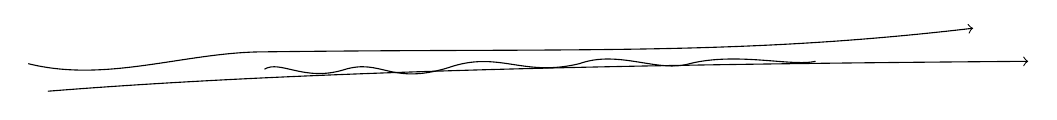
\begin{tikzpicture}
\draw[->] (0,.2)..controls(1,-.05)and(2,.35)..(3,.35)..controls(7,.4)and(9,.3)..(12,.65);
\draw[->] (.25,-.15)..controls(4,.15)and(9,.2)..(12.7,.23);
\draw (3,.13)..controls(3.2,.25)and(3.5,-.03)..(4,.12)..controls(4.5,.28)and(4.6,-.1)..(5.4,.17)..controls(6,.35)and(6.3,.03)..(7,.2)..controls(7.5,.38)and(8,.08)..(8.4,.2)..controls(9,.35)and(9.7,.16)..(10,.23);
\end{tikzpicture}}

$I$ \deleted{\illegible{1}} pol. comb. fini d'ordre $n\geq3$

``carte $n$-gonale $I$-\unsure{pondérée}

$u\in D_I$

\deleted{\[
\Pi_I=\frac{\underset{\substack{\downarrow\\\unsure{\text{libre}}\\\unsure{\text{eng. par }}I}}{L_I}}
{(\unsure{\lambda_0}\,\unsure{\lambda_i},\ \unsure{\lambda_{n-1}^{2}}=1)}
\qquad\unsure{I}\ \unsure{\text{n'est}}
\]}

\[
\Pi_I=\deleted{\unsure{L_I}}(\mathbf Z/2)^{*I}
\]
\deleted{\[
\unsure{\lambda_0}\,\underset{\unsure{n-1}}{\unsure{\lambda_i}}\,
\lambda_0\lambda_{n-1}\lambda_{\unsure{n-2}}\ldots\lambda_1=1
\]}

\diagram{\begin{tikzcd}[ampersand replacement=\&,column sep=small,row sep=large]
1\arrow[r]\&\Pi_I^+\arrow[r]\arrow[d,"\unsure{\wr|2}"']\&\Pi_I\arrow[r]\&\mathbf Z/2\arrow[r]\&1\\
\&\uline{L_I/\text{---}}\&\mathfrak S_I\&\&
\end{tikzcd}}

\figure{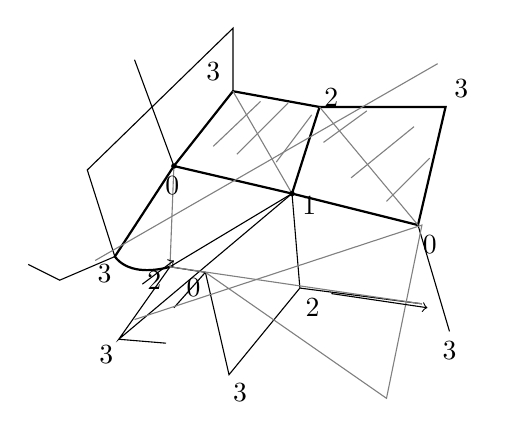
\begin{tikzpicture}[x=1cm,y=1cm]
\draw[thick] (1.2,3.3)--(1.95,4.25)--(3.05,4.05)--(2.7,2.95)--cycle;
\draw[thick] (3.05,4.05)--(4.65,4.05)--(4.3,2.55)--(2.7,2.95);
\draw (4.3,2.55)--(4.7,1.2);
\draw (2.7,2.95)--(2.8,1.75)--(4.35,1.55);
\draw (2.8,1.75)--(1.9,.65)--(1.6,1.95)--(1.15,2.02)--(2.7,2.95);
\draw[thick] (1.2,3.3)--(.45,2.15)..controls(.6,1.95)and(.9,1.95)..(1.15,2.02);
\draw (1.15,2.02)--(.5,1.1)--(2.7,2.95);
\draw (.5,1.1)--(1.1,1.05);
\draw (1.2,3.3)--(.7,4.65);
\draw (.45,2.15)--(.1,3.25)--(1.95,5.05)--(1.95,4.25);
\draw (.45,2.15)--(-.25,1.85)--(-.65,2.05);
\draw (1.6,1.95)--(1.2,1.5);
\draw[gray] (.2,2.1)--(4.55,4.6);
\draw[gray] (.7,1.35)--(4.35,2.55)--(3.9,.35)--(1.6,1.95);
\draw[gray] (1.2,3.3)--(1.15,2.02)--(4.35,1.55);
\draw[gray] (1.95,4.25)--(2.7,2.95);\draw[gray] (1.7,3.55)--(2.3,4.12);\draw[gray] (2.0,3.45)--(2.65,4.1);\draw[gray] (2.5,3.35)--(2.95,3.95);
\draw[gray] (3.05,4.05)--(4.3,2.55);\draw[gray] (3.1,3.6)--(3.65,4);\draw[gray] (3.45,3.15)--(4.25,3.8);\draw[gray] (3.9,2.85)--(4.45,3.4);
\fill (1.2,3.3) circle(.035);\fill (2.7,2.95) circle(.035);
\node at (1.18,3.05) {$0$};\node at (2.92,2.8) {$1$};\node at (3.2,4.17) {$2$};
\node at (1.7,4.5) {$3$};\node at (4.85,4.28) {$3$};\node at (4.45,2.3) {$0$};\node at (4.7,.95) {$3$};
\node at (2.96,1.5) {$2$};\node at (2.04,.42) {$3$};\node at (1.45,1.75) {$0$};\node at (.95,1.85) {$2$};\node at (.34,.9) {$3$};\node at (.32,1.93) {$3$};
\draw[->,thin] (.8,1.8)--(1.2,2.1);\draw[->,thin] (3.2,1.68)--(4.42,1.5);
\end{tikzpicture}}

\mspage{13}
